\documentclass[10pt]{article}
\usepackage{graphicx}
\usepackage{array}
\usepackage{booktabs}
\usepackage[margin=3cm, top=5cm, headheight=900pt]{geometry}
\usepackage{cmbright}
\usepackage[OT1]{fontenc}
\usepackage{float}
\usepackage[table]{xcolor}
\usepackage{pgfplots}
\pgfplotsset{compat=newest}
\usepackage{caption}
\usepackage{subcaption}
\usepackage{fancyhdr}
\usepackage{blindtext}
\usepackage{rotating}
\usepackage{tabularx}
\newcolumntype{Y}{>{\centering\arraybackslash}X}
\usepackage{amsmath}
\usepackage{natbib}
\setcitestyle{square}

\pagestyle{fancy}
\rhead{\iffloatpage{}{\includegraphics[width=0.2\textwidth]{/Users/finn/Documents/Cardiff-University-logo-for-website}}}
\lhead{\iffloatpage{}{{\large PX2155 Observational Techniques in Astronomy \\ Electronic Laboratory Diary} \\ How fast does the sun rotate? Investigating sunspots. \\ \today \\ Finnbar Wilson \vspace{0.6cm}}}
\renewcommand\headrulewidth{\iffloatpage{0pt}{0.4pt}}

\begin{document}



\section{Aims and Objectives}

In this report, data and images collected by the SOlar and Heilospheric Observatory (SOHO) from the 1$^{\text{st}}$ to the $16^{\text{th}}$ of January 2002 will be used to analyse sunspots. The latitude and longitude of several sunspots will be determined so that the sidereal period of the sun can be calculated. The relationships between latitude and period will also be analysed so that the angular momentum of the sun can be found. The values calculated in this report will then be compared to public data and journals to assess the accuracy of the experiments taking place.  

\section{Plan}
In this experiment, the subsequent outline will be followed in order to ensure that the report meets all of the scientific goals as listed below:
\begin{itemize}
	\item Import the thirteen pictures of the sun as FITS files into Gaia.
	\item Record the date time, Central x coordinate of the image, central y coordinate of the image and the radius of the sun all of which are found in the FITS file header.
	\item Identify a sunspot and determine its central x and y coordinates.
	\item Calculate the longitude and latitude of each sunspot
	\item Find the rotational period of the sun from a plot of longitude vs time. From this find the suns angular momentum
\end{itemize}
\section{Risk Assessment}
This experiment has little to no risk so it is safe to carry out the experiment.
\begin{table}[H]
	\centering
	\caption{Risk Assessment}
	\begin{tabular}{p{0.2\textwidth}p{0.65\textwidth}}
		\toprule
		Risk & Mitigation \\
		\midrule
		Tripping & Place trip hazards under desk \\
		\addlinespace
		\cellcolor{gray!10} Electric shock & \cellcolor{gray!10} Do not drink water in the lab \\
		\addlinespace
		Sitting for long period of time & Can cause wrist and band injuries so take frequent breaks to stand up and stretch. \\
		\bottomrule
	\end{tabular}
\end{table}

\newpage

\section{Context: Sunspots}

Sunspots are areas of magnetic disturbance that inhibit convection which causes a decrease in surface temperature \citep{noaa}. This magnetic disturbance is intense magnetic flux pushing up from further within the solar interior which causes localised heating in the chromosphere and photosphere, these areas are referred to as active regions. The active regions present themselves as solar plage in the chromosphere and solar facula in the photosphere as shown in figure \ref{fig:sun}.

\begin{figure}[H]
	\begin{subfigure}[t]{0.602\textwidth}
		\centering
		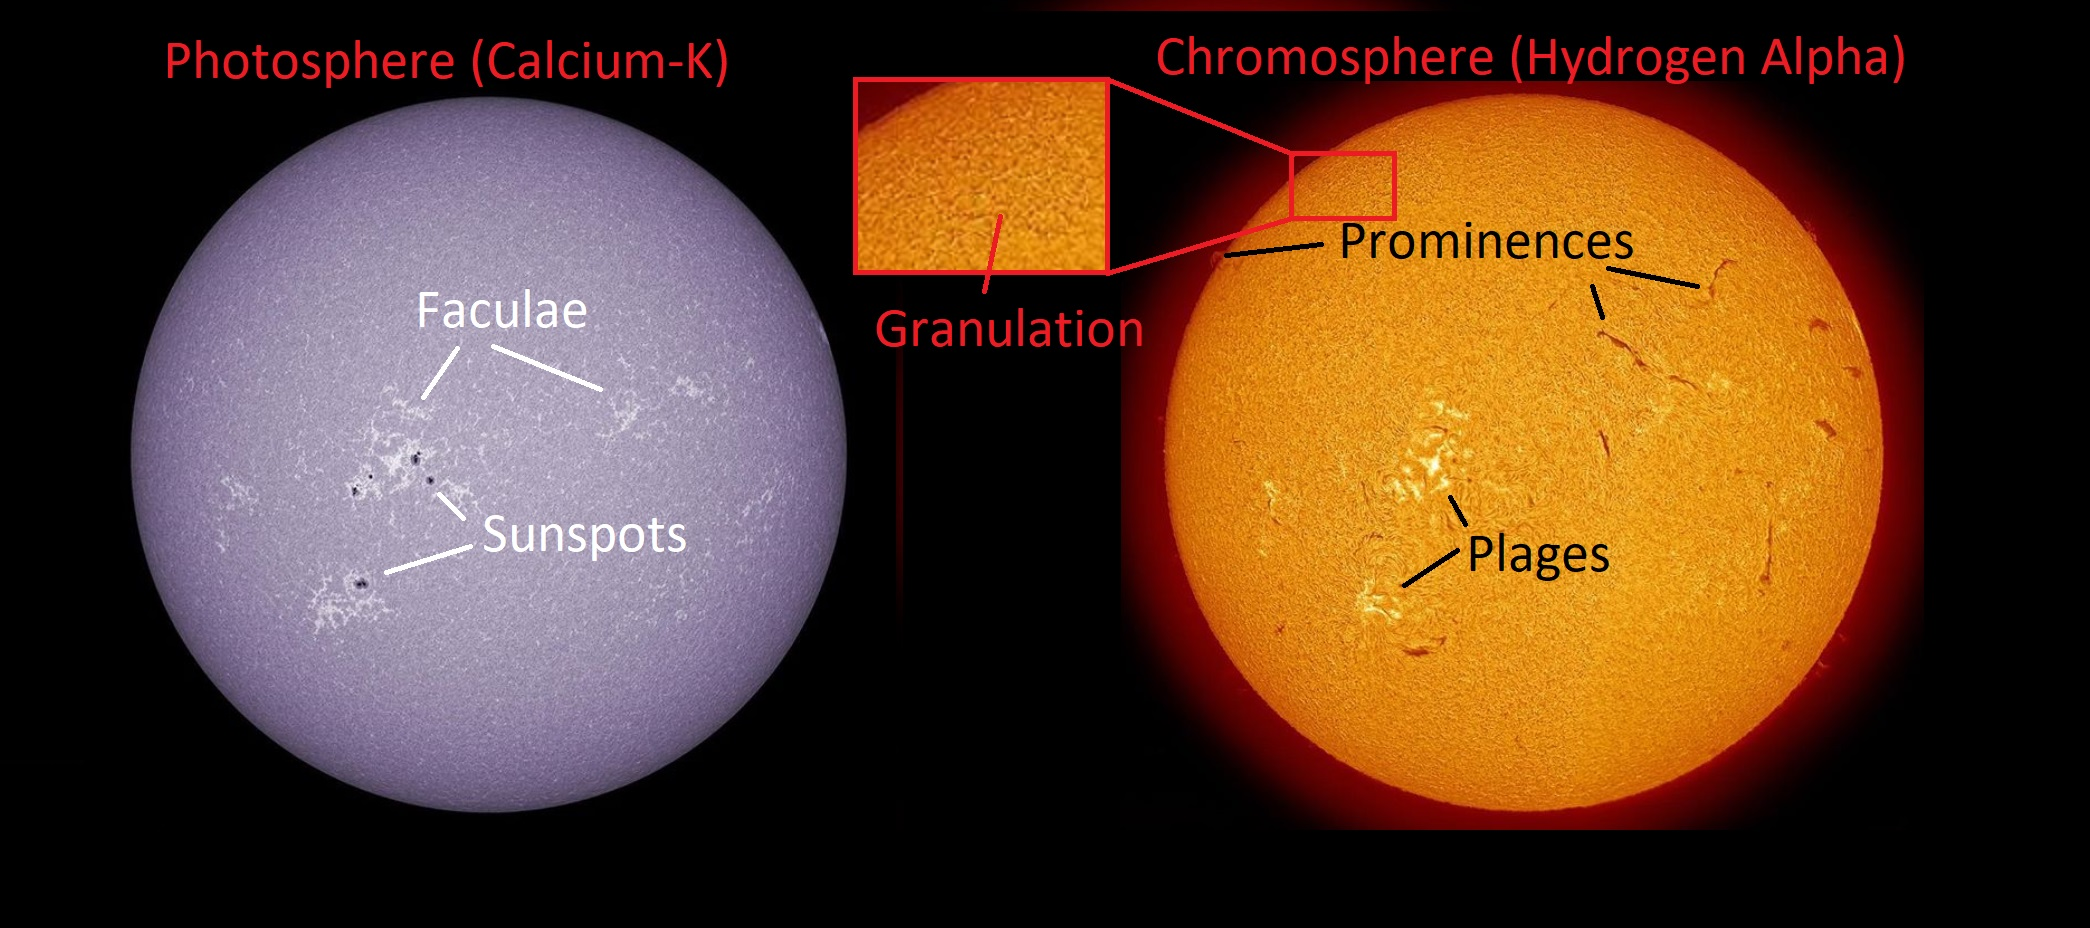
\includegraphics[width=\textwidth]{Features-on-the-Sun.jpg}
		\caption{Image by \citet{dave2018}}
		\label{fig:sun}
	\end{subfigure}
	\begin{subfigure}[t]{0.4\textwidth}
		\centering
		\includegraphics[width=\textwidth]{sunspot_dia.gif}
		\caption{Image by \citet{umbra}}
		\label{fig:umbra}
	\end{subfigure}
	\caption{Images of sunspot regions. Figure \ref{fig:sun} shows the faculae, plages and sunspots in both the photosphere and chromosphere. Figure \ref{fig:umbra} shows the umbra and penumbra of a sunspot. }
\end{figure}

\noindent There is research which has shown a relationship between plage and sunspot formation \citep{theo2022}. Sunspots are areas with temperatures of roughly 2000 kelvin cooler than the surrounding material that have two main structures: a central umbra and a surrounding penumbra. The umbra, located at the heart of the sunspot as shown in figure \ref{fig:umbra}, is the darkest and coolest part, where the magnetic field is strongest and approximately normal to the surface. Surrounding the umbra is the penumbra, a lighter and more diffuse region characterised by radial filaments extending outward which are more inclined to the magnetic field than the umbra \citep{penumbra}. Sunspots can change in size, number, and distribution over their lifetime due to the dynamic nature of the Sun's magnetic activity. Initially, sunspots often emerge in pairs with opposite magnetic polarities. As the solar cycle progresses, new sunspots tend to appear at higher latitudes, and their number increases. Eventually, the overall magnetic activity decreases, and sunspots become less frequent \citep{noaa}.

\newpage

\section{Methods}

In this experiment the position of a sunspot is recorded over time so that the period of rotation for the sun can be calculated. To do this the following method was preformed:

\begin{enumerate}
	\item Cardiff University's virtual linux system was opened and Gaia was started
	\item The thirteen pictures of the sun taken by SOHO were uploaded into Gaia and 8 sunspots were picked out in total for this experiment. A range of latitudes of the sunspots were picked. These eight randomly picked sunspots are shown in figure \ref{fig:pic}.
	\item The date time, central x-coordinate, central y-coordinate and the radius of the sun in unit of pixels were recorded into table \ref{tab:constants} from the FITS file header for each image.
	\item the x and y coordinate of the most central point of each sunspot were found and recorded into table \ref{tab:coor}. The spaces represented by - are when the sunspot could not be visible.
\end{enumerate}

\begin{figure}[H]
	\centering
	\begin{subfigure}[t]{0.244\textwidth}
		\centering
		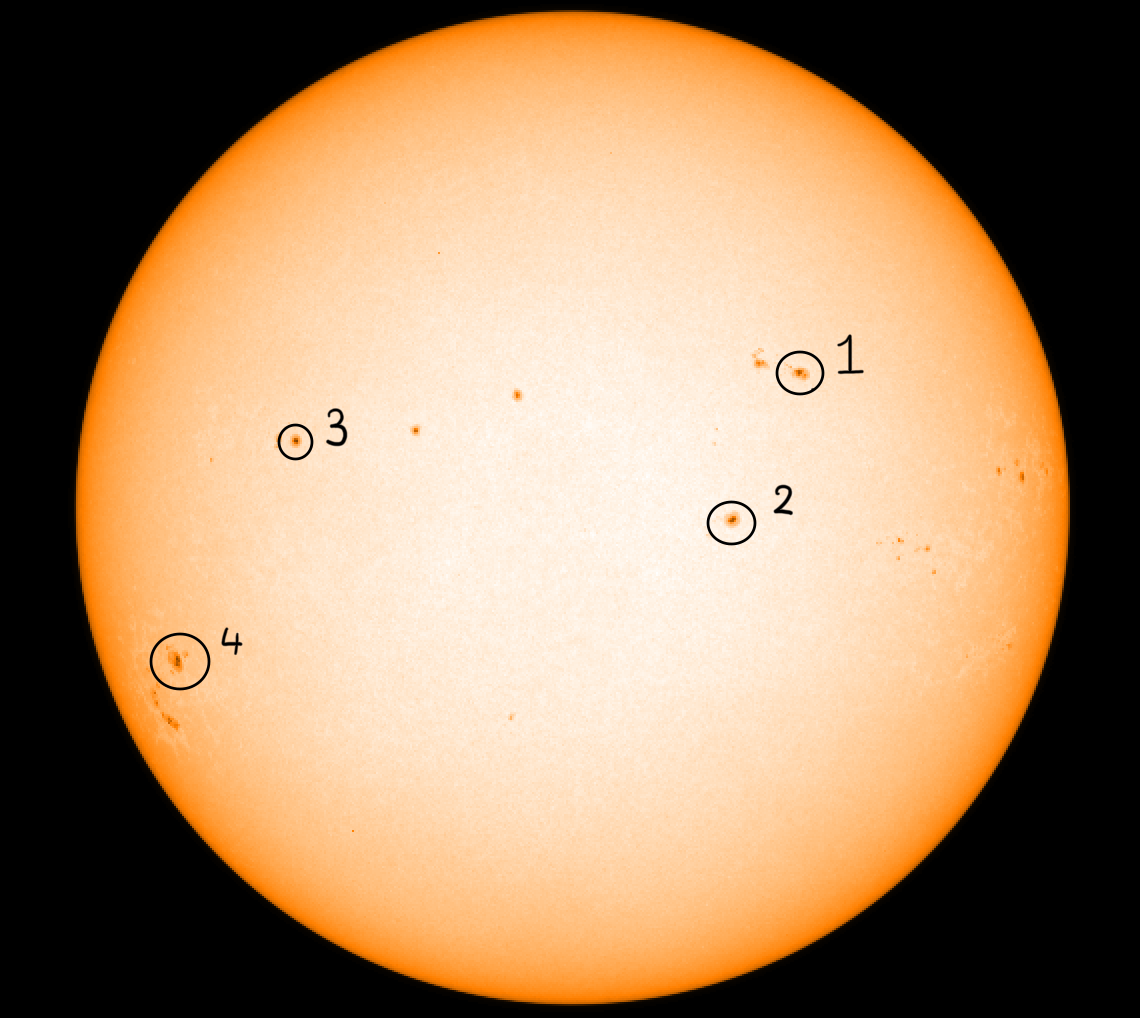
\includegraphics[width=\textwidth]{date1.png}
		\caption{2002-01-01 01:35:30}	
	\end{subfigure}
	\hfill
	\begin{subfigure}[t]{0.24\textwidth}
		\centering
		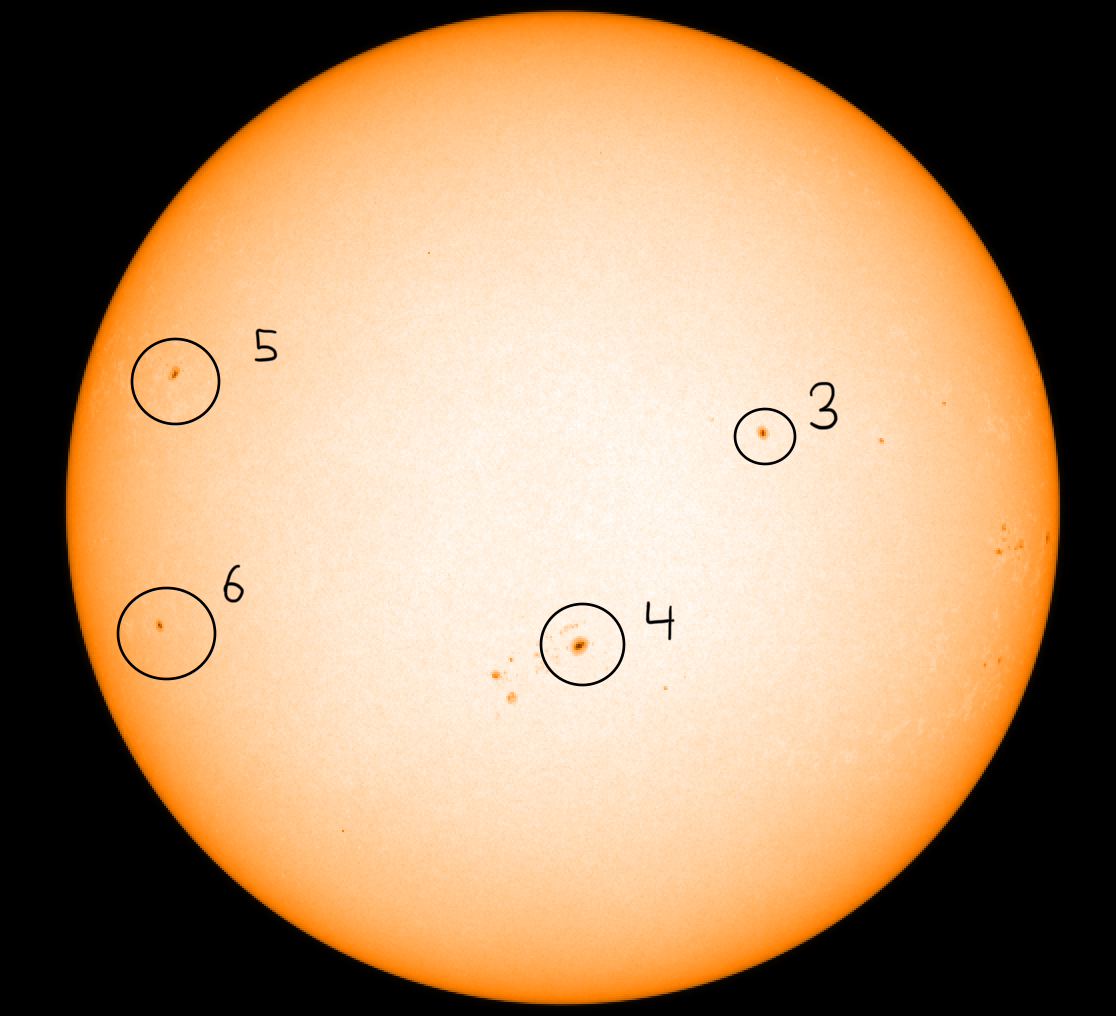
\includegraphics[width=\textwidth]{date4.png}
		\caption{2002-01-05 11:11:30}	
	\end{subfigure}
	\hfill
	\begin{subfigure}[t]{0.24\textwidth}
		\centering
		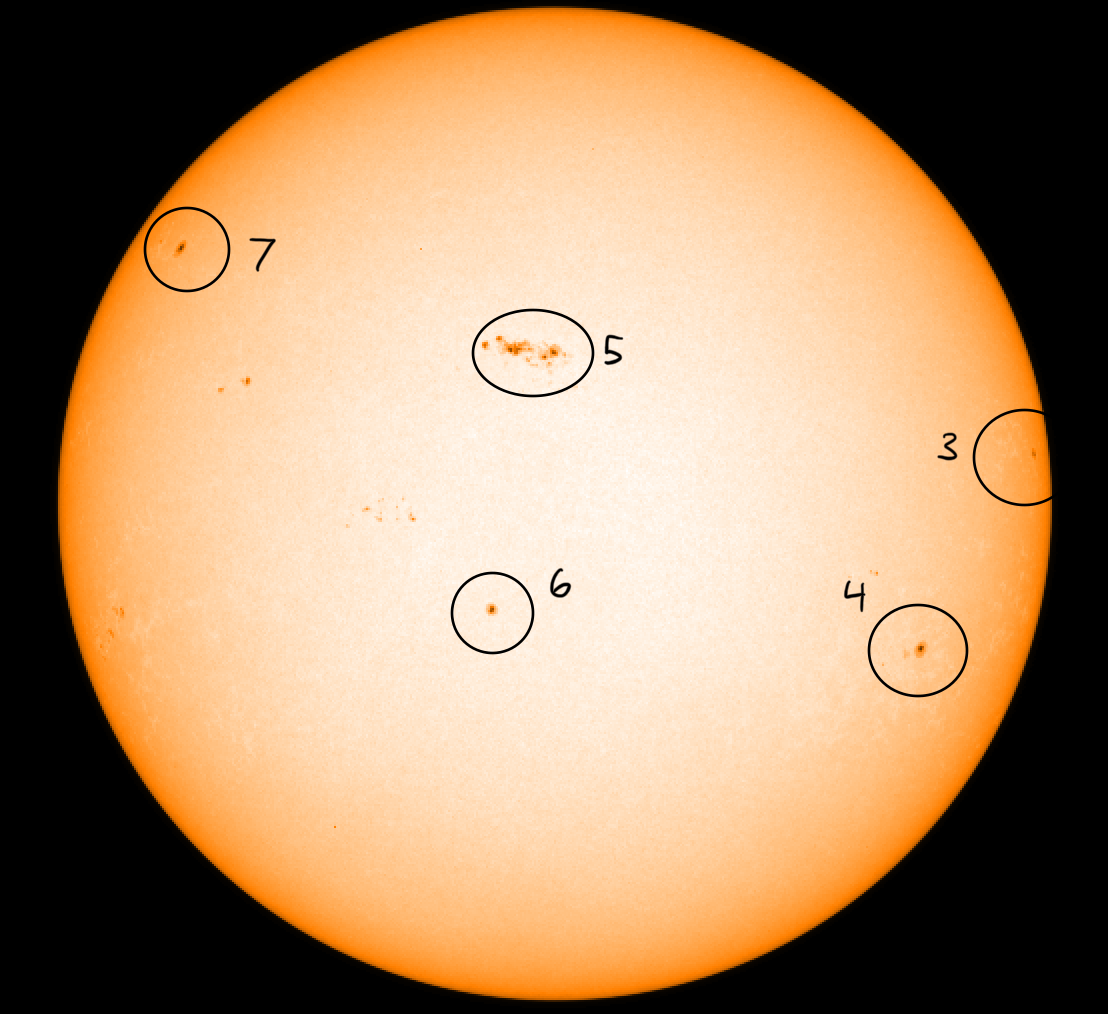
\includegraphics[width=\textwidth]{date7.png}
		\caption{2002-01-09 06:23:30}	
	\end{subfigure}
	\hfill
	\begin{subfigure}[t]{0.236\textwidth}
		\centering
		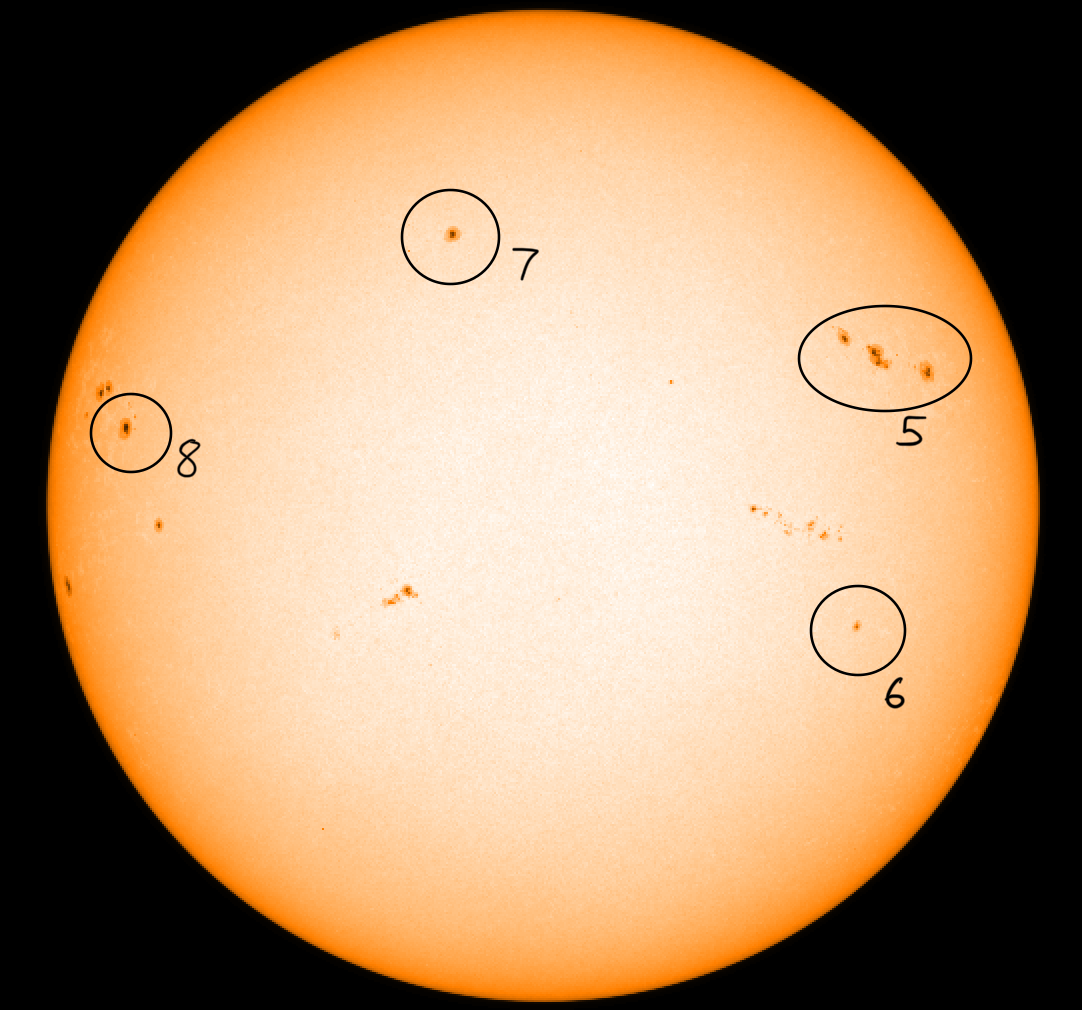
\includegraphics[width=\textwidth]{date10.png}
		\caption{2002-01-12 23:59:30}	
	\end{subfigure}
	\caption{Four of the thirteen pictures taken of the sun in January 2002. Sunspots 1-8 are shown by the black circles.}
	\label{fig:pic}
\end{figure}

\noindent Once the x and y coordinates where found for each sunspot equation \ref{eq:lat} and \ref{eq:long} were used to find their corresponding latitude and longitude in degrees for their position on the sun.

\begin{equation}
	\text{Latitude} = \sin^{-1} \left( \frac{y-\text{CENTER\_Y}}{R_{\odot}} \right)
	\label{eq:lat}
\end{equation}
Where $y$ is the y-coordinate of the sunspot, CENTER\_Y is the central y coordinate and $R_{\odot}$ is the radius of the sun in pixels.
\begin{equation}
	\text{Longitude} = \sin^{-1} \left( \frac{x-\text{CENTER\_X}}{R_{\odot}} \right)
	\label{eq:long}
\end{equation}
Where $x$ is the x-coordinate of the sunspot, CENTER\_X is the central X coordinate. The values for the longitude and latitude for each sunspot are shown in table \ref{tab:longlat}.

\begin{sidewaystable}
	\centering
	\caption{ A Table of coordinates for each sunspot}
	\begin{tabularx}{1.223\textwidth}{l|YY|YY|YY|YY|YY|YY|YY|YY}
		\toprule
		\qquad \quad Time & \multicolumn{2}{c|}{SP1} & \multicolumn{2}{c|}{SP2} & \multicolumn{2}{c|}{SP3} & \multicolumn{2}{c|}{SP4} & \multicolumn{2}{c|}{SP5} & \multicolumn{2}{c|}{SP6} & \multicolumn{2}{c|}{SP7} & \multicolumn{2}{c}{SP8} \\
		\quad y-m-d \quad \quad h:m:s & x & y & x & y & x & y & x & y & x & y & x & y & x & y & x & y\\
		\midrule
		2002-01-01 01:35:30 & 739.5 & 647.5 & 673.0 & 500.0 & 236.0 & 579.0 & 117.5 & 360.5 & - & - & - & - & - & - & - & -  \\
		2002-01-02 06:23:30 & 857.0 & 642.0 & 799.0 & 498.0 & 359.0 & 582.0 & 207.0 & 364.0 & - & - & - & - & - & - & - & - \\
		2002-01-03 20:43:30 & 959.0 & 630.0 & 927.0 & 490.0 & 537.0 & 586.0 & 361.0 & 368.0 & - & - & - & - & - & - & - & -\\
		2002-01-05 11:11:30 & - & - & - & - & 713.0 & 586.0 & 529.0 & 374.0 & 125.0 & 644.0 & 111.0 & 394.0 & - & - & - & - \\
		2002-01-06 20:27:30 & - & - & - & - & 849.0 & 580.0 & 675.0 &  376.0 & 237.0 & 652.0 & 211.0 & 402.0 & - & - & - & - \\
		2002-01-07 23:59:30 & - & - & - & - & 935.0 & 572.0 & 783.0 & 372.0 & 351.0 & 656.0 & 319.0 & 406.0 & - & - & - & -\\
		2002-01-09 06:23:30 & - & - & - & - & 993.0 & 562.0 & 879.0 & 366.0 & 471.0 & 666.0 & 451.0 & 406.0 & 139.0 & 768.0 & - & -\\
		2002-01-10 11:11:30 & - & - & - & - & - & - & 945.0 &  360.0 & 603.0 & 668.0 & 581.0 & 404.0 & 211.0 & 776.0 & - & - \\
		2002-01-11 19:11:30 & - & - & - & - & - & - & - & - & 743.0 & 664.0 & 719.0 & 400.0 & 315.0 & 780.0 & - & -\\
		2002-01-12 23:59:30 & - & - & - & - & - & - & - & - & 847.0 & 660.0 & 827.0 & 390.0 & 423.0 & 784.0 & 97.0 & 590.0\\
		2002-01-14 06:23:30 & - & - & - & - & - & - & - & - & 929.0 & 652.0 & 917.0 & 382.0 & 545.0 & 784.0 & 191.0 & 598.0\\
		2002-01-15 11:11:30 & - & - & - & - & - & - & - & - & - & - & - & - & 657.0 & 784.0 & 307.0 & 606.0\\
		2002-01-16 17:35:30 & - & - & - & - & - & - & - & - & - & - & - & - & 767.0 & 778.0 & 447.0 & 610.0\\
		\bottomrule
	\end{tabularx}
	\caption*{The first column is time in the format year-month-day hour:minute:seconds. The rest of the columns represent each sunspot from 1 to 8 and their respective x and y coordinates in the units of pixels.}
	\label{tab:coor}
	\vspace{1mm}
	\caption{A table of longitude and latitude of each sunspot}
	\begin{tabularx}{1.223\textwidth}{l|YY|YY|YY|YY|YY|YY|YY|YY}		
		\toprule
		\qquad \quad Time & \multicolumn{2}{c|}{SP1} & \multicolumn{2}{c|}{SP2} & \multicolumn{2}{c|}{SP3} & \multicolumn{2}{c|}{SP4} & \multicolumn{2}{c|}{SP5} & \multicolumn{2}{c|}{SP6} & \multicolumn{2}{c|}{SP7} & \multicolumn{2}{c}{SP8} \\
		\quad y-m-d \quad \quad h:m:s & lat & long & lat & long & lat & long & lat & long & lat & long & lat & long & lat & long & lat & long\\
		\midrule
		2002-01-01 01:35:30 &  +15.8 &  +27.1 & -1.4 &  +18.8 &  +7.7 & -33.8 & -17.7 & -52.5 &  - &  - &  - &  - &  - &  - &  - &  - \\
		2002-01-02 06:23:30 &  +15.1 &  +43.8 & -1.6 &  +35.1 &  +8.1 & -18.0 & -17.3 & -37.9 &  - &  - &  - &  - &  - &  - &  - &  - \\
		2002-01-03 20:43:30 &  +13.7 &  +63.7 & -2.6 &  +56.3 &  +8.5 &  +2.8 & -16.8 & -17.8 &  - &  - &  - &  - &  - &  - &  - &  - \\
		2002-01-05 11:11:30 &  - &  - &  - &  - &  +8.5 &  +23.7 & -16.1 &  +1.9 &  +15.4 & -51.2 & -13.7 & -53.8 &  - &  - &  - &  - \\
		2002-01-06 20:27:30 &  - &  - &  - &  - &  +7.8 &  +42.5 & -15.9 &  +19.0 &  +16.3 & -33.7 & -12.8 & -37.4 &  - &  - &  - &  -\\ 
		2002-01-07 23:59:30 &  - &  - &  - &  - &  +6.9 &  +58.0 & -16.4 &  +32.9 &  +16.8 & -19.0 & -12.3 & -22.9 &  - &  - &  - &  -\\ 
		2002-01-09 06:23:30 &  - &  - &  - &  - &  +5.7 &  +74.8 & -17.1 &  +47.4 &  +18.0 & -4.8 & -12.3 & -7.1 &  +30.9 & -48.7 &  - &  - \\
		2002-01-10 11:11:30 &  - &  - &  - &  - &  - &  - & -17.8 &  +60.3 &  +18.2 &  +10.4 & -12.6 &  +7.9 &  +32.0 & -37.4 &  - &  - \\
		2002-01-11 19:11:30 &  - &  - &  - &  - &  - &  - &  - &  - &  +17.8 &  +27.5 & -13.0 &  +24.4 &  +32.6 & -23.5 &  - &  - \\
		2002-01-12 23:59:30 &  - &  - &  - &  - &  - &  - &  - &  - &  +17.3 &  +42.2 & -14.2 &  +39.1 &  +33.1 & -10.4 &  +9.0 & -56.8\\ 
		2002-01-14 06:23:30 &  - &  - &  - &  - &  - &  - &  - &  - &  +16.3 &  +56.8 & -15.2 &  +54.3 &  +33.1 &  +3.7 &  +9.9 & -40.3 \\
		2002-01-15 11:11:30 &  - &  - &  - &  - &  - &  - &  - &  - &  - &  - &  - &  - &  +33.1 &  +16.8 &  +10.9 & -24.4 \\
		2002-01-16 17:35:30 &  - &  - &  - &  - &  - &  - &  - &  - &  - &  - &  - &  - &  +32.3 &  +30.7 &  +11.3 & -7.6 \\
		\bottomrule
	\end{tabularx}
	\caption*{The first column is time in the format year-month-day hour:minute:seconds. The rest of the columns represent each sunspot from 1 to 8 and their respective values for longitude and latitude in the units of degrees.}
	\label{tab:longlat}
\end{sidewaystable}

\newpage

\section{Results and discussion}

%The longitude in degrees recored in table \ref{tab:longlat} was plotted vs time in days in figure \ref{fig:long}.

\begin{figure}[H]
	\centering
	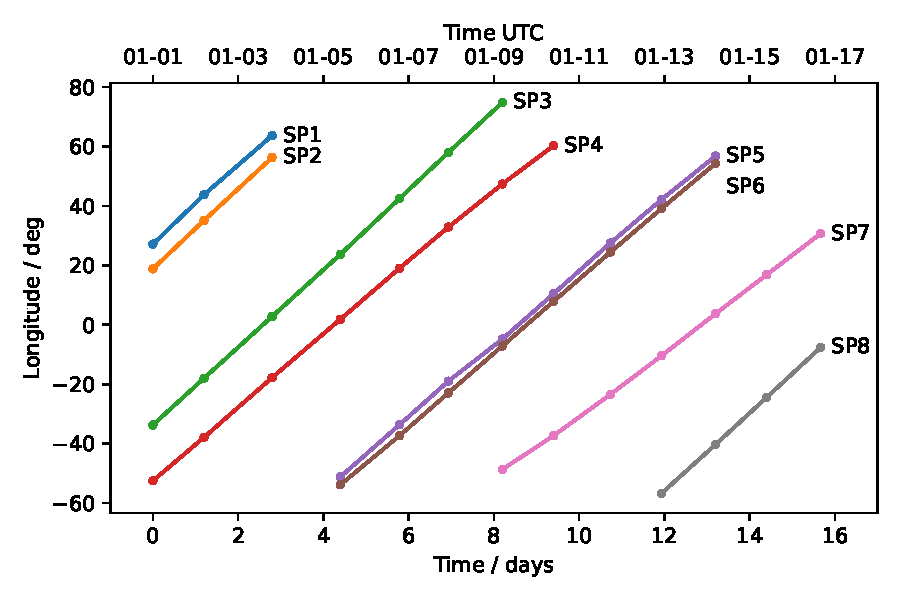
\includegraphics[width = 0.75\columnwidth]{daytime.pdf}
	\caption{A plot of the longitude of each sun spot in degrees vs time. The bottom axis represents time in days from the first image. The top axis represents the UTC time. A linear line of best fit was used for each of the sunspots, each of which produced a gradient represented by $\frac{d}{dt} ( \text{Longitude} )$ in table \ref{tab:period}.}
	\label{fig:long}
\end{figure}

\noindent Each of the lines of best fit in figure \ref{fig:long} are linear and have a gradient $\frac{d}{dt} ( \text{Longitude} )$ which is expected as the sun rotates at a constant velocity. Given that for one full rotation of the sun it spins 360 degrees longitudinally, so by extrapolating the equations of line of best fit the period of rotation can be calculated. This is shown by equation \ref{eq:period}.

\begin{equation}
	P = \frac{360}{\frac{d}{dt} ( \text{Longitude} )}
	\label{eq:period}
\end{equation}

\noindent The $\frac{d}{dt} ( \text{Longitude} )$ for each sunspot is shown in table \ref{tab:period} as well as its synodic period in days.

\begin{table}[H]
	\centering
	\caption{table of synodic period of rotation for each sunspot}
	\begin{tabularx}{0.6\textwidth}{XXr}
		\toprule
		Sunspot &  $\frac{d}{dt} ( \text{Longitude} )$ & Period/Days \\
		\midrule
		SP1 & $ 13.0 \pm  1.1$ & $ 27.6 \pm  2.2$ \\
		SP2 & $ 13.4 \pm  0.8$ & $ 26.9 \pm  1.5$ \\
		SP3 & $ 13.2 \pm  0.7$ & $ 27.2 \pm  1.5$ \\
		SP4 & $ 12.1 \pm  0.7$ & $ 29.8 \pm  1.7$ \\
		SP5 & $ 12.3 \pm  0.7$ & $ 29.3 \pm  1.6$ \\
		SP6 & $ 12.4 \pm  0.7$ & $ 29.1 \pm  1.5$ \\
		SP7 & $ 10.7 \pm  0.6$ & $ 33.6 \pm  2.0$ \\
		SP8 & $ 13.2 \pm  0.7$ & $ 27.3 \pm  1.5$ \\
		\bottomrule
	\end{tabularx}
	\label{tab:period}
\end{table}

\noindent The average latitude in degrees was calculated from the data in table \ref{tab:longlat} by taking the mean value with an uncertainty of $\pm$ its range. The sidereal period of the sun can be calculated by using equation \ref{eq:sidereal}.

\begin{equation}
	P_{\text{sidereal}} = \frac{P \times 365.25}{P + 365.25}
	\label{eq:sidereal}
\end{equation}

\noindent The average latitude of each sunspot and its sidereal period is recorded in table \ref{tab:sideperiod}.

\begin{table}[H]
	\centering
	\caption{table of sidereal period of rotation for each sunspot}
	\begin{tabularx}{0.6\textwidth}{lYr}
		\toprule
		Sunspot &  Average latitude/deg & Sidereal Period/Days \\
		\midrule
		SP1 & $ 14.9 ^{+ 0.9} _{-1.2} $ & $ 25.7 \pm  2.2$ \\
		\addlinespace
		SP2 & $-1.9 ^{ +0.5} _{-0.7} $ & $ 25.0 \pm  1.5$ \\
		\addlinespace
		SP3 & $ 7.6 ^{ +0.9} _{-1.9} $ & $ 25.3 \pm  1.5$ \\
		\addlinespace
		SP4 & $-16.9 ^{ +1.0} _{-0.9} $ & $ 27.5 \pm  1.7$ \\
		\addlinespace
		SP5 & $ 17.0 ^{+ 1.2} _{-1.6} $ & $ 27.1 \pm  1.6$ \\
		\addlinespace
		SP6 & $-13.3 ^{ +1.0} _{-1.9} $ & $ 27.0 \pm  1.5$ \\
		\addlinespace
		SP7 & $ 32.4 ^{+ 0.7} _{-1.5} $ & $ 30.8 \pm  2.0$ \\
		\addlinespace
		SP8 & $ 10.3 ^{ +1.1} _{-1.3} $ & $ 25.4 \pm  1.5$ \\
		\bottomrule
	\end{tabularx}
	\label{tab:sideperiod}
\end{table}

\noindent A plot of average latitude in degrees vs sidereal period in days is shown in figure \ref{fig:lat}.

\begin{figure}[H]
	\centering
	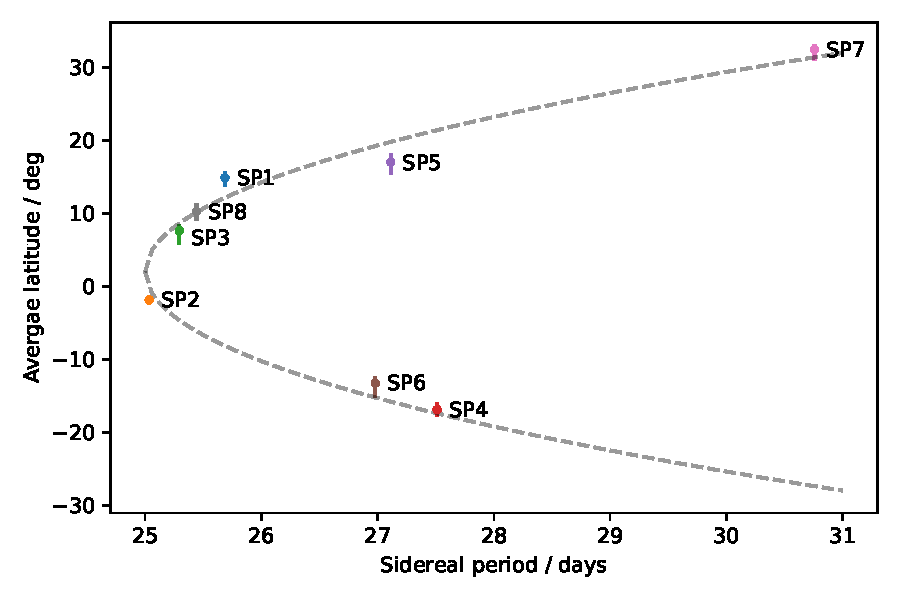
\includegraphics[width = 0.75\columnwidth]{period.pdf}
	\caption{A plot of the data from table \ref{tab:sideperiod}. The error bars represent the range of latitude values that were used to calculate the average latitude. The grey dashed line is used to show how the sidereal period of the sun calculations vary with the latitude of the sunspot used. It has the equation: $(y-2)^2 = 150x - 3750$.}
	\label{fig:lat}
\end{figure}

\noindent Figure \ref{fig:lat} shows that the calculated sidereal period of increases the further from the equator the sunspot is. This could partially be due to the parallax error when trying to find the coordinates of a point on a sphere in 2d. This parallax error would be at a minimum at the equator and maximum at the poles. Another solution to this occurrence is that different latitudes of the sun rotate at different speeds, \citet{Beck2000} suggests that since the sun is non rigid (gaseous) it can have differential rotation. \\\\
Using the equation $(y-2)^2 = 150x - 3750$ that represents the dashed grey line in figure \ref{fig:lat} and that $y=$ latitude and $x=$ period, the sidereal period of rotation at the equator (latitude = 0$^{\circ}$) is 25 days and at the poles (latitude = $\pm 45^{\circ}$) is 39 days. This is in agreement with \citet{latrotation}. The equation also contains the component $(y-2)$, This suggests that the suns rotation axis is roughly tilted by 2$^{\circ}$ from the axis of earth orbit. This value is not in agreement with \citet{dwilliams} who suggest the value is 7.25$^{\circ}$. Given that the equation that found this value is untested on other data sets it is more likely that \citet{dwilliams} has a more accurate value. The angular momentum of the sun can be found using equation \ref{eq:angular}.
\begin{equation}
	L = I \omega
	\label{eq:angular}
\end{equation}
Where \qquad \qquad \qquad $I = (2/5)M_{\odot}(R_{\odot}^2)$ \qquad \qquad and \qquad \qquad $\omega = \frac{2 \pi}{P(\text{seconds})}$ \\

\noindent$I$ is the moment of inertia of a sphere and $\omega$ is its angular velocity. Assuming that the period is 25 days then the angular momentum of the sun is $( 1.12 \pm 0.09)\times 10^{42}$ kg m$^2$ s$^{-1}$. This value is not in agreement with \citet{cang} which found it to be $1.88 \times 10^{41}$ kg m$^2$ s$^{-1}$. The period of 25 days was used here as it is the predicted period of rotation at the equator found from figure \ref{fig:lat}. \\

\noindent Comment on errors/uncertainties: During the recording of the data the only uncertainty was in the x and y coordinate values. When finding the central point within the sunspot there is an uncertainty of $\pm$ the range of pixels the sunspot took, for most of the sunspots this was roughly $\pm$ 10 pixels in x and y. This uncertainty is not represented in table \ref{tab:coor} but was included in the error calculations for all subsequent values derived from them. Another source of uncertainty is in the linear plotting function (least square method) used to find $\frac{d}{dt} ( \text{Longitude} )$ of each sunspot. This uncertainty is included table \ref{tab:period}.

\section{Conclusion}

In this report, data and images from the SOlar and Heilospheric Observatory (SOHO) were used to analyse the position, longitude and latitude, of 8 randomly picked sunspots. By tracking the movement of sunspots across the solar surface, The sidereal period of each sunspot was calculated. A plot of average latitude vs sidereal period was then made which found that the sidereal period of the sunspot increased with the latitude of the sunspot which agrees with both \citet{Beck2000} and \citet{latrotation}. The equation $(\text{Latitude}-2)^2 = 150\times P_{\text{sidereal}} - 3750$ models this relationship. The angular momentum of the sun around its axis of rotation was then found to be $( 1.12 \pm 0.09)\times 10^{42}$ kg m$^2$ s$^{-1}$ which is not in agreement with \citet{cang}. This report has analysed the rotational behaviour of the sun and provided insights into the mechanisms of sunspots however it could not accurately calculate the angular momentum of the sun.

\bibliographystyle{agsm}
\bibliography{sunspotref}

\section*{Appendix}

\begin{table}[H]
	\centering
	\caption{Constants of each FITS file}
	\begin{tabularx}{0.6\textwidth}{lYYY}
		\toprule
		Time & CENTER\_X & CENTER\_Y & $R_{\odot}$ \\
		\midrule
		2002-01-01 01:35:30 &  512.5 &  512.2 &  497.6 \\
		2002-01-02 06:23:30 &  512.6 &  512.2 &  497.6 \\
		2002-01-03 20:43:30 &  513.0 &  512.2 &  497.6 \\
		2002-01-05 11:11:30 &  512.8 &  512.2 &  497.6 \\
		2002-01-06 20:27:30 &  512.9 &  512.2 &  497.6 \\
		2002-01-07 23:59:30 &  512.9 &  512.2 &  497.6 \\
		2002-01-09 06:23:30 &  512.7 &  512.2 &  497.6 \\
		2002-01-10 11:11:30 &  512.9 &  512.2 &  497.5 \\
		2002-01-11 19:11:30 &  513.1 &  512.2 &  497.5 \\
		2002-01-12 23:59:30 &  513.1 &  512.3 &  497.5 \\
		2002-01-14 06:23:30 &  512.8 &  512.3 &  497.5 \\
		2002-01-15 11:11:30 &  512.8 &  512.3 &  497.4 \\
		2002-01-16 17:35:30 &  513.1 &  512.3 &  497.4 \\
		\bottomrule
	\end{tabularx}
	\caption*{Time in the format year-month-day hour:minute:seconds, CENTER\_X, CENTER\_Y and $R_{\odot}$ are in the unit pixels. }
	\label{tab:constants}
\end{table}

\end{document}
